\documentclass[portrait,final,a0paper]{baposter}
%\documentclass[a4shrink,portrait,final]{baposter}
% Usa a4shrink for an a4 sized paper.

\tracingstats=2
\usepackage{calc}
\usepackage{graphicx}
\usepackage{amsmath}
\usepackage{amssymb}
\usepackage{relsize}
\usepackage{multirow}
\usepackage{bm}

\usepackage{graphicx}


\usepackage{pgfbaselayers}
\pgfdeclarelayer{background}
\pgfdeclarelayer{foreground}
\pgfsetlayers{background,main,foreground}

\usepackage{times}
\usepackage{helvet}
%\usepackage{bookman}
\usepackage{palatino}
\usepackage{background}

\newcommand{\captionfont}{\footnotesize}

\selectcolormodel{cmyk}

\graphicspath{{images/}}


%%%%%%%%%%%%%%%%%%%%%%%%%%%%%%%%%%%%%%%%%%%%%%%%%%%%%%%%%%%%%%%%%%%%%%%%%%%%%%
%%% Begin of Document
%%%%%%%%%%%%%%%%%%%%%%%%%%%%%%%%%%%%%%%%%%%%%%%%%%%%%%%%%%%%%%%%%%%%%%%%%%%%%%


\begin{document}
\typeout{Poster rendering started}	

\SetBgContents{}
%%% Setting Background Image %%%%%%%%%%%%%%%%%%%%%%%%%%%%%%%%%%%%%%%%%%%%%%%%%%
\background{
	\begin{tikzpicture}[remember picture,overlay]%
	\draw (current page.center)+(-1em,1em) node[anchor=center,opacity=0.2, scale=1.1]
	{\includegraphics[width=1.1\textwidth]{background1}};
	\end{tikzpicture}
}	

%%%%%%%%%%%%%%%%%%%%%%%%%%%%%%%%%%%%%%%%%%%%%%%%%%%%%%%%%%%%%%%%%%%%%%%%%%%%%%
%%% Here starts the poster
%%%---------------------------------------------------------------------------
%%% Format it to your taste with the options
%%%%%%%%%%%%%%%%%%%%%%%%%%%%%%%%%%%%%%%%%%%%%%%%%%%%%%%%%%%%%%%%%%%%%%%%%%%%%%
% Define some colors
\definecolor{DarkMagenta}{cmyk}{0,0.64,0.2,0}
\definecolor{yellow}{cmyk}{0.3,0.1,0.2,0.0}
\definecolor{reddishyellow}{cmyk}{0,0.22,1.0,0.0}
\definecolor{black}{cmyk}{0,0,0.0,1.0}
\definecolor{darkYellow}{cmyk}{0,0,1.0,0.5}
\definecolor{Carnelian}{cmyk}{1.0,0.29,0.0,0.26}

\definecolor{lightyellow}{cmyk}{0.0,0.0,0.0,0.0}
\definecolor{lighteryellow}{cmyk}{0,0,0.0,0.0}
\definecolor{lighteryellow}{cmyk}{0,0,0.0,0.0}
\definecolor{lightestyellow}{cmyk}{0,0,0.0,0.0}

\definecolor{primary1}{cmyk}{0.5,1.0,0.0,0.0}
\definecolor{primary2}{cmyk}{0,0,0,0.5}
\definecolor{primary3}{cmyk}{0,0,0,0.8}

\definecolor{secondary1}{cmyk}{0.82,0.38,0.2,0.2}
\definecolor{secondary2}{cmyk}{0.91,0.91,0.6,0.18}
\definecolor{secondary3}{cmyk}{0.71,0.23,0.13,0.3}
\definecolor{secondary4}{cmyk}{0.38,0.16,0.0,0.0}
\definecolor{secondary5}{cmyk}{0.20,0.62,0.2,0.0}
\definecolor{secondary6}{cmyk}{0.63,0.2,0.26,0.0}

%%
%\typeout{Poster Starts}

\newlength{\leftimgwidth}
\begin{poster}%
  % Poster Options
  {
  % Show grid to help with alignment
  grid=false,
  % Column spacing
  colspacing=1em,
  % Color style
  bgColorOne=lightestyellow,
  bgColorTwo=lightestyellow,
  borderColor=primary2,
  headerColorOne=primary1,
  headerColorTwo=reddishyellow,
  headerFontColor=white,
  boxColorOne=lightyellow,
  boxColorTwo=lighteryellow,
  % Format of textbox
  textborder=roundedleft,
%  textborder=rectangle,
  % Format of text header
  eyecatcher=false,
  headerborder=open,
  headerheight=0.095\textheight,
  headershape=roundedright,
  headershade=plain,
  headerfont=\Large\sf\bf, %Sans Serif
 % boxshade=plain,
%  background=shade-tb,
  background=user,
  linewidth=1.6pt
  }
  % Eye Catcher
  {\includegraphics[width=10em]{background1.png}} % No eye catcher for this poster. (eyecatcher=no above). If an eye catcher is present, the title is centered between eye-catcher and logo.
  % Title
  {
  \vspace{2.2em}
  \color{primary1}
  \textbf{
  Classification of Cells Based on Scale-space Features and Semi-supervised Machine Learning}
  }
  % Authors
  {
  % Serif
  \vspace{0.5em}\textbf{\ S. Vohra\textsuperscript{2}, L. Antanas\textsuperscript{2}, L. Raedt\textsuperscript{2} and D. Prodanov\textsuperscript{1}}\\
   \textsuperscript{1}EHS, Imec, Leuven, Belgium, \textsuperscript{2} DTAI, KU Leuven\\
   \vspace{1.94em}
    
  }
  % University logo
  {% The makebox allows the title to flow into the logo, this is a hack because of the L shaped logo.  
  	 \makebox[11em][r]{%
  	 	\begin{minipage}{16em}
  	 		\hfill
  	 		
\includegraphics[height=7.8em]{imec_logo}
  	 	\end{minipage}
  	 }
  }
   
    
%%%%%%%%%%%%%%%%%%%%%%%%%%%%%%%%%%%%%%%%%%%%%%%%%%%%%%%%%%%%%%%%%%%%%%%%%%%%%%
%%% Now define the boxes that make up the poster
%%%---------------------------------------------------------------------------
%%% Each box has a name and can be placed absolutely or relatively.
%%% The only inconvenience is that you can only specify a relative position 
%%% towards an already declared box. So if you have a box attached to the 
%%% bottom, one to the top and a third one which should be in between, you 
%%% have to specify the top and bottom boxes before you specify the middle 
%%% box.
%%%%%%%%%%%%%%%%%%%%%%%%%%%%%%%%%%%%%%%%%%%%%%%%%%%%%%%%%%%%%%%%%%%%%%%%%%%%%%
    %
 
%%%%%%%%%%%%%%%%%%%%%%%%%%%%%%%%%%%%%%%%%%%%%%%%%%%%%%%%%%%%%%%%%%%%%%%%%%%%%%
  \headerbox{Motivation}{name=contribution,column=2,row=0, span=1}{
%%%%%%%%%%%%%%%%%%%%%%%%%%%%%%%%%%%%%%%%%%%%%%%%%%%%%%%%%%%%%%%%%%%%%%%%%%%%%%
\begin{itemize}
	\item Experts segment Anatomical \& Time Lapse Images manually.
	\item Tools in literature are very domain specific. 
	\item Most of the tools are based on original intensity which varies alot among images. 
\end{itemize}
	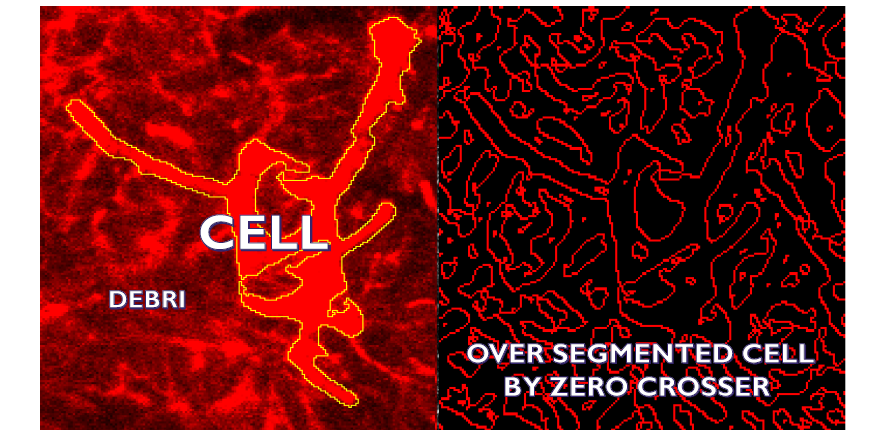
\includegraphics[width=7.2cm, height=2.8cm]{tool}	
	\color{secondary1}\textbf{Example of ZeroCrosser for Segmentation }	

}


%%%%%%%%%%%%%%%%%%%%%%%%%%%%%%%%%%%%%%%%%%%%%%%%%%%%%%%%%%%%%%%%%%%%%%%%%%%%%%

\headerbox{Problem Outline}{name=funding,column=0,span=2,row=0}{
	%%%%%%%%%%%%%%%%%%%%%%%%%%%%%%%%%%%%%%%%%%%%%%%%%%%%%%%%%%%%%%%%%%%%%%%%%%%%%%
		\begin{minipage}{.30\textwidth}
			 \textbf{ SUPERVISED LEARNING} 
				\begin{itemize}
				\color{Carnelian} 	\item MultiClass Problem		
				\end{itemize}
			  \textbf{INSTANCE}
				\begin{itemize}
			   \color{Carnelian} 	\item Pixel Characterized By Feature Vector							
				\end{itemize}
					
		\end{minipage} 
		\begin{minipage}{.70\textwidth}
			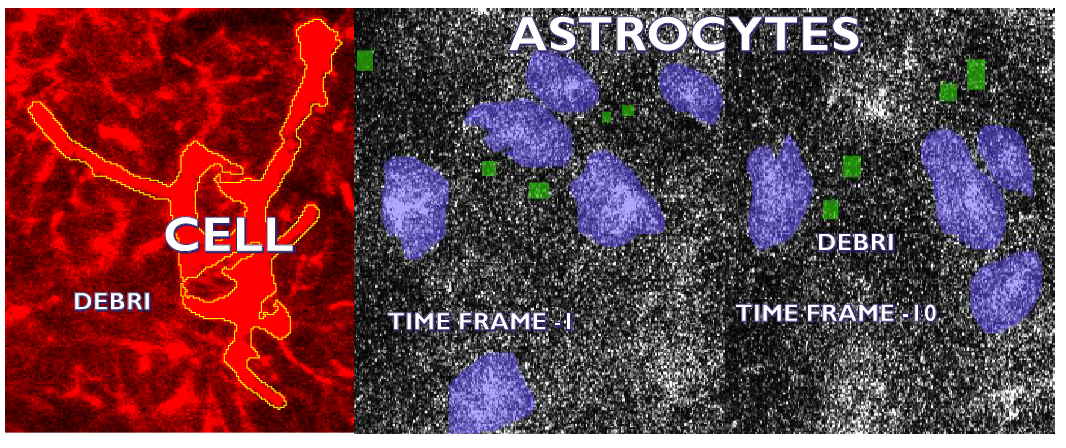
\includegraphics[width=10.5cm, height=3.5cm ]{MONTAGE31}
		\end{minipage}
	\newline 	
	\textbf{OBJECTIVE} 	\color{primary1}\hspace{2.7cm}\textbf{ANATOMICAL IMAGE }	 \hspace{1.2cm}\textbf{TIME LAPSE IMAGES}	
	\color{black}
	\begin{itemize}
		\item Build an interactive framework that adapts to every learning task without assumption's  about number of classes and types of objects represented.
		\item "Learning by example" given like  \color{primary1}debris around cell, \color{secondary1}cytoplasm, \color{primary1}nucleus \color{black} etc.		
     	\item Segment images in an objective manner.
	\end{itemize}	
}

%%%%%%%%%%%%%%%%%%%%%%%%%%%%%%%%%%%%%%%%%%%%%%%%%%%%%%%%%%%%%%%%%%%%%%%%%%%%%%
  \headerbox{Features Extraction }{name=feature,column=0,below=contribution,span=3}{
%%%%%%%%%%%%%%%%%%%%%%%%%%%%%%%%%%%%%%%%%%%%%%%%%%%%%%%%%%%%%%%%%%%%%%%%%%%%%%
	\begin{minipage}{.11\textwidth}	
		\color{Carnelian}\textbf{FILTERS} 
		\newline  
		\newline
		\color{black}\textbf{Gaussian }
		\newline
		\newline	
		\textbf{Gaussian X,Y}
		\newline 	
		\textbf{Derivatives} 
		\newline 
		\newline 
		\newline 
		\textbf{Laplace of} 
		\newline 
		\textbf{Gaussian}
		\newline  
		\newline
		\newline
		\textbf{BiLaplace of} 	
		\newline 
		\textbf{Gaussian}
	\end{minipage}
\begin{minipage}{.13\textwidth}  
  	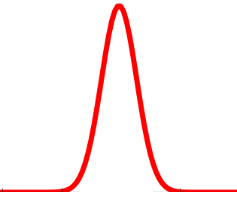
\includegraphics[width=2.5cm, height=1.6cm]{gaussian}
  	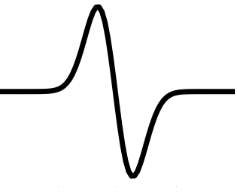
\includegraphics[width=2.5cm, height=1.6cm]{gaussiand}
  	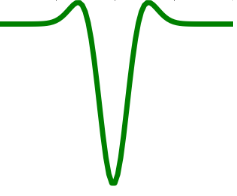
\includegraphics[width=2.5cm, height=1.6cm]{LOG}
  	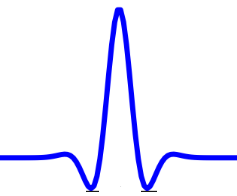
\includegraphics[width=2.5cm, height=1.6cm]{BLOG}	
\end{minipage}
\begin{minipage}{.10\textwidth}
    
\includegraphics[width=1.3cm, height=1.2cm]{convolution1}
    
\includegraphics[width=1.3cm, height=1.2cm]{convolution2}
    \newline 
    \color{primary1}\textbf{Region}
    \newline 
    \color{primary1} \hspace{0.3cm}\textbf{Of}
    \newline
    \textbf{Interest}
    
\includegraphics[width=1.5cm, height=1.2cm]{convolution3}
    
\includegraphics[width=1.5cm, height=1.2cm]{convolution4}
\end{minipage}
\begin{minipage}{.18\textwidth}
\color{primary1} \hspace{0.1cm}\textbf{CONVOLVED ROI}
\newline
\textbf{AT VARIOUS SCALES}
\newline
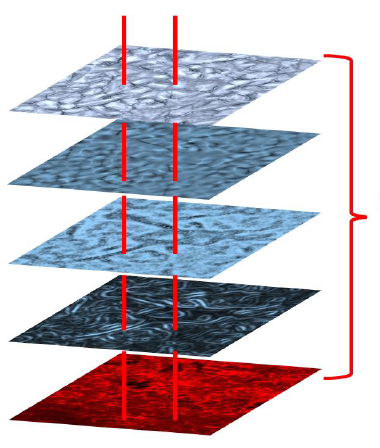
\includegraphics[width=4.1cm, height=5.8cm]{filteredImage}	
\end{minipage}
\begin{minipage}{.18\textwidth}
	\color{black}\textbf{MULTIDIMENSIONAL}
	\newline
	\color{black}\hspace{0.3cm}\textbf{FEATURE VECTOR}
	\newline
	\color{black}\hspace{0.3cm}\textbf{ OF EACH PIXEL}
	\newline
	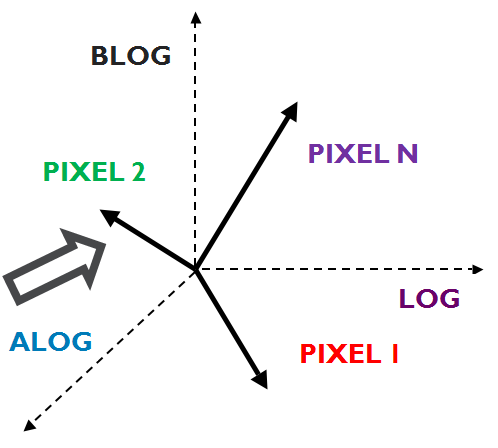
\includegraphics[width=4.2cm, height=2.9cm]{vector}	
    \color{primary1} \hspace{1.5cm}\textbf{$\bigoplus$}
	\newline
	\color{Carnelian} \hspace{0.5cm}\textbf{CLASS LABEL}
	\newline
    \color{Carnelian} \hspace{0.3cm}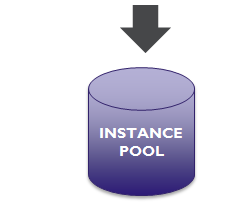
\includegraphics[width=2.5cm, height=1.8cm]{pool}	
\end{minipage}
 \begin{minipage}{.30\textwidth}
 	 \color{primary1} \textbf{MULTISCALE FILTER RESPONSE}
 	    \newline
 		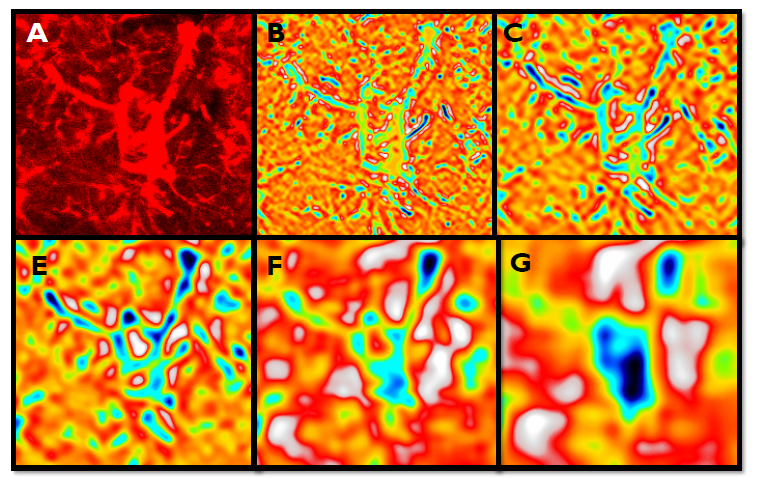
\includegraphics[width=6.8cm, height=5.3cm]{LOGMONTAGE1}
 		\newline
 		\color{secondary2} 
 		\textbf{A}: Initial Image. 
 		\newline
 		\textbf{B-F}: Laplace of Gaussian, i.e. Mexican hat
 		\newline
 		\textbf{SCALE}: 2,4,8,16,32.
 \end{minipage} 
  }

%%%%%%%%%%%%%%%%%%%%%%%%%%%%%%%%%%%%%%%%%%%%%%%%%%%%%%%%%%%%%%%%%%%%%%%%%%%%%%
\headerbox{ Comparision between Thresholding \& Learning }{name=baseline,column=0,span=3,below=feature}{
\color{primary1}\textbf{THRESHOLDING}\hspace{7.5cm}\textbf{VOTING}\hspace{4.5cm}\textbf{ACTIVE LEARNING} 
\newline 
\begin{minipage}{.36\textwidth}
\text{}
\newline 
\color{black}\text{Objects can be separated from each other by selecting}
\newline
\text{a Threshold value minimizing a cost function}
\newline 
\color{primary1}\hspace{1.2cm}\textbf{LOCAL}\hspace{3.3cm}\textbf{GLOBAL} 
\newline 
\color{Carnelian}\hspace{0.2cm}\text{Different threshold values}\hspace{0.7cm}\text{One threshold value}
\newline 
\color{Carnelian}\hspace{0.4cm}\text{for each Scale \& Filter}\hspace{1.5cm}\text{for each Scale}
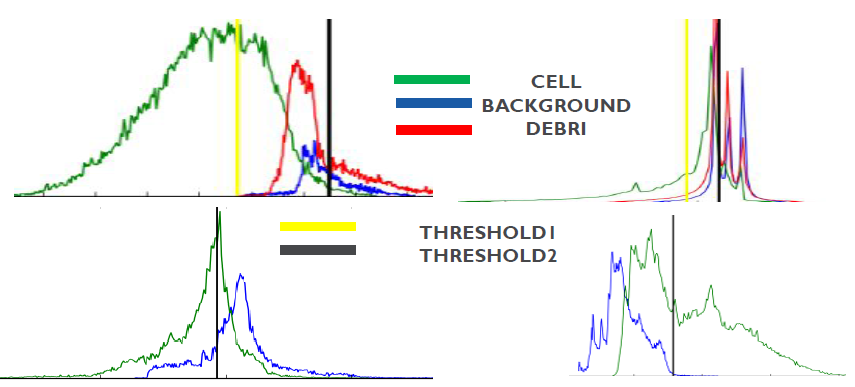
\includegraphics[width=.90\textwidth]{threshold14T}
\end{minipage}
\begin{minipage}{.25\textwidth}
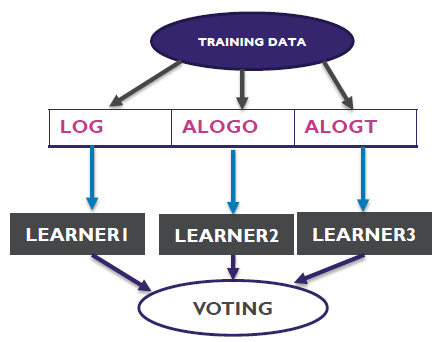
\includegraphics[width=5.9cm, height=5.3cm]{voting}	
\end{minipage} 
\begin{minipage}{.40\textwidth}
\color{black}\text{Interactively collect new training examples by querying}
\newline 
\text{human user}
\newline
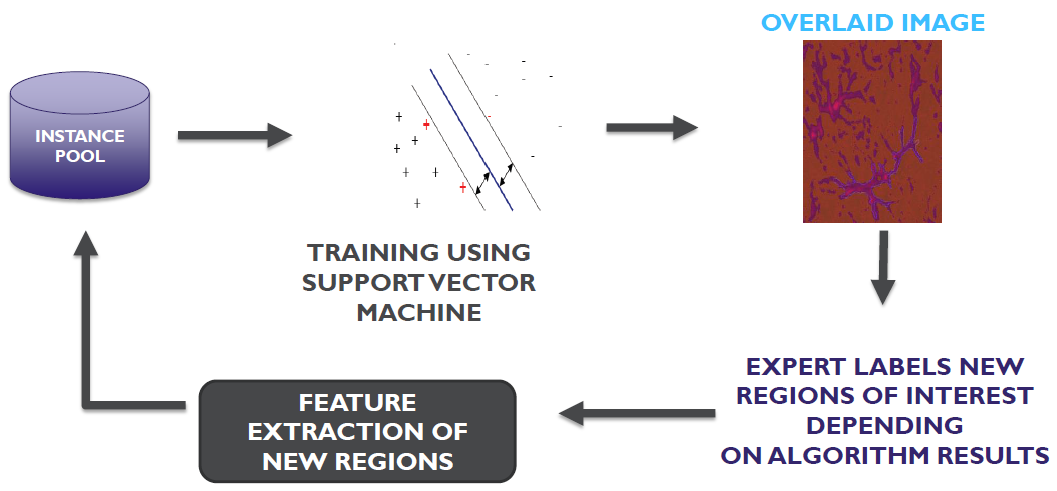
\includegraphics[width=0.97\textwidth]{activelearning2}	
\end{minipage} 						
}

\headerbox{Comparision Results}{name=evaluation,column=0,span=2,below=baseline}{
	\color{primary1} \textbf{EXTERNAL VALIDATION}\hspace{3.9cm} \textbf{ROC \& PR CURVES SVM APPROACH}
	\newline
			\begin{minipage}{.13\textwidth}	
				\textbf{}		 
				\color{primary1}\newline\text{Anatomical }
				\text{Image} 
				\color{black}
				\newline	
				\newline
				\text{Background} 	
				\text{Cell} 
				\newline 
				\text{Debri} 	
				\newline 
				\text{Avg} 
				\newline 
				\color{primary1}\text{Time Lapse}
				\text{Images}
				\color{black}
				\newline 
				\text{Background} 
				\newline 
				\text{Astrocytes} 
				\text{Avg} 	
			\end{minipage}
		\begin{minipage}{.47\textwidth}
			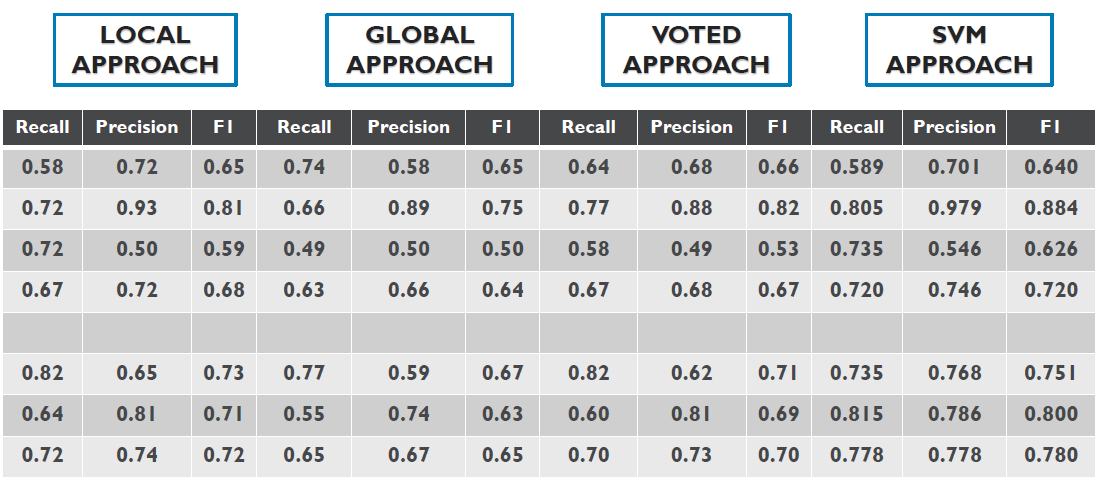
\includegraphics[width=6.8cm, height=4.9cm]{results125T}
		\end{minipage} 		
		\begin{minipage}{.40\textwidth}
			\includegraphics[width=5.8cm, height=4.9cm ]{results134}
		\end{minipage}	
}
  \headerbox{Summary \& Conclusion}{name=conclusion,column=2,span=1,below=baseline}{
  	%%%%%%%%%%%%%%%%%%%%%%%%%%%%%%%%%%%%%%%%%%%%%%%%%%%%%%%%%%%%%%%%%%%%%%%%%%%%%%
  	Presented Approach is 
  	\begin{itemize}
  		\item \color{primary1}\textbf{Task Independent: } \color{black}not only limited to one specific task.
  		\item \color{primary1}\textbf{Cell Type Independent: }\color{black} not only limited to specific type of cell.
  	\end{itemize} 
  \color{Carnelian}	Future efforts will include implementing the Structural SVM or Relational Learning for finding the suitable patterns in astrocytic arbors.
  }
	\hspace{6 cm}
 \centerline{ 
 	\begin{minipage}{20em}
 		
\includegraphics[height=1.5em]{logo_kul}   		
 		\vspace{0.1cm}		
 	\end{minipage}
 		\begin{minipage}{20em}
 			
\includegraphics[height=2.4em]{imec_logo}   		
 			\vspace{0.1cm}		
 		\end{minipage}
 }

\end{poster}

\end{document}
